\section{Experimental analysis}
\label{sec:analysis}

\subsection{Analysis strategy and event selection}
\label{subsec:analysis}
This search is focused on the $\ttbar A \to W^+b W^- \bar{b}b\bar{b}$ process, with one of the $W$ bosons
decaying leptonically and the other $W$ boson decaying hadronically. Only electrons or muons originating 
from $W$ boson or $\tau$-lepton decays are considered. The resulting final state signature is thus characterised
by one electron or muon, and high jet and $b$-jet multiplicity that can be exploited to suppress the background,
dominated by $\ttbar$+jets production. Therefore, the following preselection requirements are made:
one electron or muon, $\geq$5 AKT4 jets and $\geq$3 AKT2 $b$-tagged jets, in the following simply referred
to as $\geq$5 jets and $\geq$3 $b$-tags. In order to optimise the sensitivity of the search, the selected events 
are categorised into two separate channels depending on the number of $b$-tags (3 and $\geq$4).
The channel with $\geq$5 jets and $\geq 4$ $b$-tags has the largest signal-to-background ratio and 
therefore drives the sensitivity of the search. It is dominated by $\ttbar$+HF background. The channel with 3 $b$-tags 
has significantly lower signal-to-background ratio and the background is enriched in $\ttbar$+light-jets.
The simultaneous analysis of both channels is particularly useful to calibrate {\sl in-situ} the $\ttbar$+jets background prediction 
(including its heavy-flavour content) and constrain the related systematic uncertainties, as it will be discussed in
Sec.~\ref{sec:stat_analysis}. This is a common strategy used in many experimental searches in the 
ATLAS and CMS collaborations~\cite{Aad:2015gra,Khachatryan:2015ila,Aad:2015kqa}, 
which we mimic here in order to obtain more realistic projected sensitivities.

%%%%%%%%%%%%%%%%%%%%%%%%%%%%%%%%%%%%%%%
\begin{figure}[htbp]
\begin{center}
\begin{tabular}{cc}
\includegraphics[width=0.4\textwidth]{Figures/DRbb.eps} &
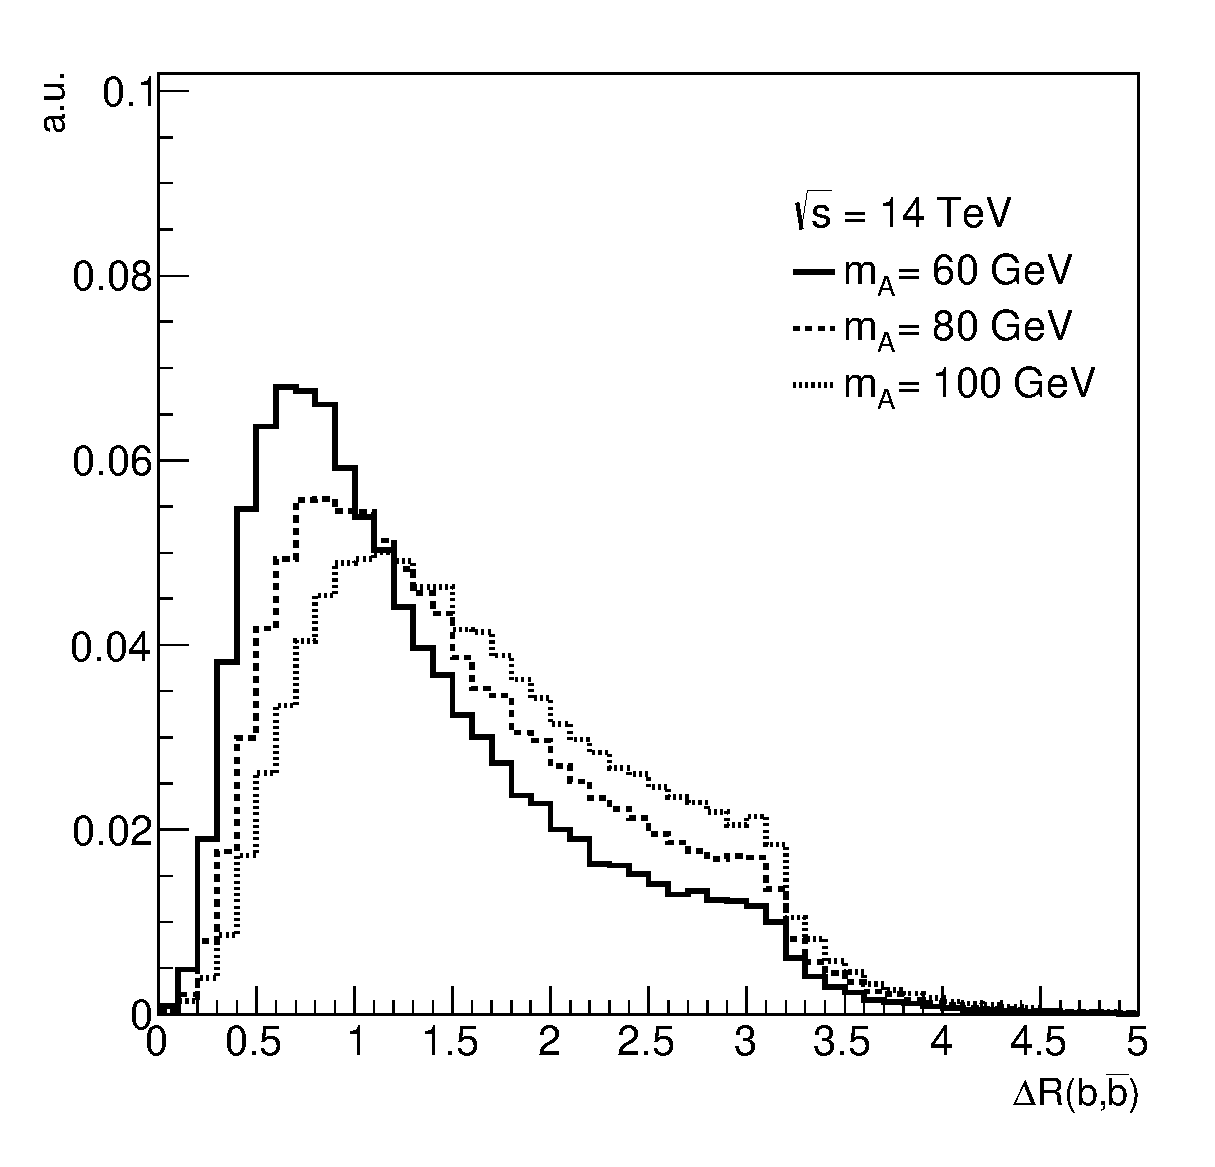
\includegraphics[width=0.4\textwidth]{Figures/DRbb2.eps} \\
(a) & (b) \\
\end{tabular}
\caption{\small {Distribution of $\Delta R$ between the two $b$-quarks from the $A \to b\bar{b}$ decay prior to
any selection requirements, for different values of $m_A$: (a) $m_A=20, 30$ and  40 GeV, and (b) $m_A=60, 80$ and 100 GeV.}}
\label{fig:DRbb_ttA} 
\end{center}
\end{figure}
%%%%%%%%%%%%%%%%%%%%%%%%%%%%%%%%%%%%%%%%%%%%%%%%%% 

An extra handle is provided by the significant boost of the $A$ boson in a fraction of signal 
events, which results in the two $b$-jets from the $A \to b\bar{b}$ decay emerging with small angular separation between them.
This is particularly relevant for low $m_A$ values, as shown in Fig.~\ref{fig:DRbb_ttA}.
As a result, the $A$ boson decay products can be reconstructed into a single fat jet, whose mass distribution would show a 
resonant structure peaked at the correct $m_A$ value. This feature is also very powerful to discriminate against the background.
Therefore, a further requirement is made to have at least one C/A BDRS-filtered jet with radius parameter $R^{\rm CA}$ and minimum $\pt$
depending on the $m_A$ hypothesis being tested. In order to correctly reconstruct a significant fraction of the signal while rejecting as 
much background as possible,  CA6 jets are used for $m_A \leq 40$ GeV, while CA8 jets are used for higher $m_A$ values (up to 100 GeV). 
The minimum $\pt$ requirements on the C/A jets are 60, 100, 120, 150, 200 and 250 GeV for
$m_A=20, 30, 40, 60, 80$ and 100 GeV, respectively. 
As shown in Fig.~\ref{fig:DRbb_ttA}, for high values of $m_A$ only a small fraction of signal events would have the $A$ decay products contained
within the CA8 jet. The small signal acceptance comes with the benefit of improved background rejection and
the ability to reconstruct the $A$ boson mass, desirable in such simple analysis. However, it is expected that a dedicated multivariate 
analysis focused on the sample rejected by this analysis, similar in spirit to the ATLAS and CMS searches for the SM Higgs boson in 
$t\bar{t} h$, $h \to b\bar{b}$~\cite{Aad:2015gra,Khachatryan:2015ila}, could also achieve significant signal sensitivity at high $m_A$. 
Evaluating this possibility is beyond the scope of this study.
The number of $b$-tags inside the C/A jet is determined by
matching the $b$-tagged AKT2 jets within a cone of radius $\Delta R =0.75 R^{\rm C/A}$. 
Finally, a requirement is made is that the C/A jets have $\geq$ 2 $b$-tags inside. In case of more than one selected C/A jet,
the leading $\pt$ one is chosen. 

Table~\ref{tab:yields} presents the expected yields for signal and the SM backgrounds 
per fb$^{-1}$ of integrated luminosity as a function of the selection cuts applied in each
of the analysis channels under consideration: ($\geq$5j, 3b) and ($\geq$5j, $\geq$4b).
In the case of the ($\geq$5j, 3b) channel, the dominant background after final selection
is $\ttbar$+light-jets, where typically the two $b$-quarks from the  top quark decays, as well as
the $c$-quark from the $W \to c\bar{s}$ decay, are $b$-tagged.
In contrast, in the ($\geq$5 j, $\geq$4 b) channel half of the background is $\ttbar$+$\geq$$1b$,
with $\ttbar$+$b\bar{b}$ being its leading contribution. The rest of the background is approximately 
equally split between $\ttbar$+$\geq$$1c$ and $\ttbar$+light-jets.
In this table the expected contribution from $\ttbar A$ signal is obtained under the assumptions of $g_t=2$ and ${\cal B}(A\to b\bar{b})=1$.
Both analysis channels have approximately the same amount of signal, while the background
is about a factor of four higher in the ($\geq$5j, 3b) channel than in the  ($\geq$5j, $\geq$4b) channel.
Together with the different composition of the background, the very different signal-to-background
ratio between both channels is the primary motivation for analysing them separately.

The final discriminating variable is the invariant mass of the selected C/A jet, referred to as 
``leading BDRS jet mass". Figures~\ref{fig:mA_1} and~\ref{fig:mA_2} show the expected distribution of the BDRS jet mass
for signal and background in each of the analysis channels, for the different $m_A$ values considered. The distributions
correspond to $\sqrt{s}=14$ TeV and are normalised to an integrated luminosity of 30 fb$^{-1}$.
For the assumed values of $g_t=2$ and ${\cal B}(A\to b\bar{b})=1$, the signal is clearly visible
on top of the background.

%%%%%%%%%%%%%%%%%%%%%%%%%%%%%%%%%%%%%%%
\begin{table}[h] 
\begin{center} 
\begin{tabular}{ccccc|cc} 
\hline\hline
&$\quad$$\ttbar$+$\geq$$1b$$\quad$ &$\quad$$\ttbar$+$\geq$$1c$$\quad$&$\quad$$\ttbar$+light-jets$\quad$&$\quad$$\ttbar+X$$\quad$ & $\quad$Total bkg.$\quad$ & $\quad$$\ttbar A$$\quad$ \\ 
\hline\hline
\multicolumn{7}{c}{$m_A=30$~GeV} \\
\hline
1 lepton&$4167$&$10958$&$155648$&$299$&$171072$&$377$ \\ 
$\geq$5 jets&$3109$&$7678$&$61866$&$215$&$72868$&$268$ \\ 
\hline
3 $b$-tags&$766$&$765$&$2702$&$30.1$&$4263$&$72.4$ \\ 
$\geq$1 CA6 jets &$510$&$502$&$1485$&$21.4$&$2518$&$55.7$ \\ 
$\geq$2 $b$-tags in selected CA6 jet & $45.1$&$38.4$&$159$&$1.9$&$\bf 245$&$\bf 14.6$ \\ 
\hline
$\geq$4 $b$-tags&$234$&$100$&$128$&$10.6$&$474$&$28.7$ \\ 
$\geq$1 CA6 jets&$171$&$70.1$&$75.7$&$7.9$&$325$&$23.8$ \\ 
$\geq$2 $b$-tags in selected CA6 jet &$36.9$&$13.2$&$18.5$&$1.5$&$\bf 70.2$&$\bf 11.7$ \\ 
\hline\hline
\multicolumn{7}{c}{$m_A=80$~GeV} \\
\hline
1 lepton&$4167$&$10958$&$155648$&$299$&$171072$&$240$ \\ 
$\geq$5 jets&$3109$&$7678$&$61866$&$215$&$72868$&$198$ \\ 
\hline
3 $b$-tags&$766$&$765$&$2702$&$30.1$&$4263$&$57.5$ \\ 
$\geq$1 CA8 jets &$252$&$246$&$646$&$11.5$&$1155$&$23.6$ \\ 
$\geq$2 $b$-tags in selected CA8 jet &$32.3$&$32.8$&$125$&$2.0$&$\bf 192$&$\bf 6.1$ \\ 
\hline
$\geq$4 $b$-tags&$234$&$100$&$128$&$10.6$&$474$&$25.0$ \\ 
$\geq$1 CA8 jets&$91.6$&$36.4$&$35.0$&$4.3$&$167$&$11.6$ \\ 
$\geq$2 $b$-tags in selected CA8 jet &$25.8$&$10.6$&$12.6$&$1.5$&$\bf 50.4$&$\bf 5.3$ \\ 
\hline\hline
\end{tabular} 
\caption{\small {Expected signal and SM backgrounds at $\sqrt{s}=14$ TeV
per fb$^{-1}$ of integrated luminosity as a function of the selection cuts applied in each
of the analysis channels under consideration (see text for details): ($\geq$5j, 3b) and ($\geq$5j, $\geq$4b).
The signal prediction is obtained under the assumptions of $g_t=2$ and ${\cal B}(A\to b\bar{b})=1$.
Several background categories have been merged for readability. The sum of 
$\ttbar$+$W$, $\ttbar$+$Z$ and $\ttbar$+$h_{\rm SM}$ is denoted as $\ttbar$+$X$. 
The yields shown correspond to the optimised selections for two different values
of $m_A$, 30 GeV and 80 GeV. Shown in bold are the signal and backgrounds
expectations after full selection in each of the analysis channels considered.}}
\label{tab:yields} 
\end{center} 
\end{table} 
%%%%%%%%%%%%%%%%%%%%%%%%%%%%%%%%%%%%%%%

%%%%%%%%%%%%%%%%%%%%%%%%%%%%%%%%%%%%%%%
\begin{figure}[htbp]
\begin{center}
\begin{tabular}{ccc}
$m_A = 20$~GeV & $m_A = 30$~GeV &  $m_A = 40$~GeV \\
\includegraphics[width=0.3\textwidth]{Figures/21stJuly/tta20/VD_1.eps} &
\includegraphics[width=0.3\textwidth]{Figures/21stJuly/tta30/VD_1.eps} &
\includegraphics[width=0.3\textwidth]{Figures/21stJuly/tta40/VD_1.eps} \\
\includegraphics[width=0.3\textwidth]{Figures/21stJuly/tta20/VD_2.eps} &
\includegraphics[width=0.3\textwidth]{Figures/21stJuly/tta30/VD_2.eps} &
\includegraphics[width=0.3\textwidth]{Figures/21stJuly/tta40/VD_2.eps} \\
\end{tabular}
\caption{\small {Distribution of the leading BDRS jet mass in the two analysis channels considered after final selection: 
(top) ($\geq$5j, 3b) and (bottom) ($\geq$5j, $\geq$4b), for different values of $m_A$ (20, 30 and 40 GeV).
The prediction corresponds to $\sqrt{s}=14$ TeV and an integrated luminosity of 30 fb$^{-1}$.
Several background categories have been merged for visibility. The expected contribution from 
the $\ttbar A$ signal under the assumptions of $g_t=2$ and ${\cal B}(A\to b\bar{b})=1$  is also shown
(red histogram), stacked on top of the SM background. The dashed red line shows the $\ttbar A$  signal 
distribution normalised to the background yield to better compare the shape to that of the background.
The bottom panel displays the expected total systematic uncertainty on the total prediction prior to the fit 
to the pseudo-data.}}
\label{fig:mA_1} 
\end{center}
\end{figure}
%%%%%%%%%%%%%%%%%%%%%%%%%%%%%%%%%%%%%%%%%%%%%%%%%% 

%%%%%%%%%%%%%%%%%%%%%%%%%%%%%%%%%%%%%%%
\begin{figure}[htbp]
\begin{center}
\begin{tabular}{ccc}
$m_A = 60$~GeV & $m_A = 80$~GeV &  $m_A = 100$~GeV \\
\includegraphics[width=0.3\textwidth]{Figures/21stJuly/tta60/VD_1.eps} &
\includegraphics[width=0.3\textwidth]{Figures/21stJuly/tta80/VD_1.eps} &
\includegraphics[width=0.3\textwidth]{Figures/21stJuly/tta100/VD_1.eps} \\
\includegraphics[width=0.3\textwidth]{Figures/21stJuly/tta60/VD_2.eps} &
\includegraphics[width=0.3\textwidth]{Figures/21stJuly/tta80/VD_2.eps} &
\includegraphics[width=0.3\textwidth]{Figures/21stJuly/tta100/VD_2.eps} \\
\end{tabular}
\caption{\small {Distribution of the leading BDRS jet mass in the two analysis channels considered after final selection: 
(top) ($\geq$5j, 3b) and (bottom) ($\geq$5j, $\geq$4b), for different values of $m_A$ (60, 80 and 100 GeV).
The prediction corresponds to $\sqrt{s}=14$ TeV and an integrated luminosity of 30 fb$^{-1}$.
Several background categories have been merged for visibility. The expected contribution from 
the $\ttbar A$ signal under the assumptions of $g_t=2$ and ${\cal B}(A\to b\bar{b})=1$  is also shown
(red histogram), stacked on top of the SM background. The dashed red line shows the $\ttbar A$  signal 
distribution normalised to the background yield to better compare the shape to that of the background.
The bottom panel displays the expected total systematic uncertainty on the total prediction prior to the fit 
to the pseudo-data.}}
\label{fig:mA_2} 
\end{center}
\end{figure}
%%%%%%%%%%%%%%%%%%%%%%%%%%%%%%%%%%%%%%%%%%%%%%%%%% 

\subsection{Systematic uncertainties}
\label{sec:systematics}

Several sources of systematic uncertainty are considered that can affect the normalisation of signal 
and background and/or the shape of the BDRS jet mass distribution. 
Individual sources of systematic uncertainty are considered uncorrelated.  Correlations of a given 
systematic uncertainty are maintained across processes and analysis channels. 
The choices of what uncertainties to consider and their magnitude are inspired by recent 
$\ttbar$+$h_{\rm SM}$, $h_{\rm SM}\to b\bar{b}$ searches at the LHC~\cite{Aad:2015gra}.

A 15\% normalisation uncertainty is assigned to $\ttbar$+light-jets corresponding to the modelling of the jet multiplicity 
spectrum. A 30\% normalisation uncertainty is assigned to each of the $\ttbar$+HF components ($\ttbar$+$b$, 
$\ttbar$+$b\bar{b}$, $\ttbar$+$B$, $\ttbar$+$c$, $\ttbar$+$c\bar{c}$, $\ttbar$+$C$), and taken to be uncorrelated among 
them. These uncertainties are expected to be conservative given the recent progress in NLO predictions for $\ttbar$ with
up to two jets merged with a parton shower~\cite{Hoeche:2014qda}, as well as NLO predictions for $\ttbar$+$\geq 1b$ production 
in the 4F scheme matched to a parton shower~\cite{Cascioli:2013era}. Cross section uncertainties for $\ttbar$+$W$, $\ttbar$+$Z$ and
$\ttbar$+$h_{\rm SM}$ are taken to be 30\% for each process. Uncertainties associated to jet energy and mass calibration are taken
to be 5\% per jet, fully correlated between energy and mass and across all jets in the event. Finally, uncertainties on the
$b$-, $c$- and light-jet tagging efficiencies are taken to be 3\%, 6\% and 15\% respectively. These uncertainties are taken 
as uncorrelated between $b$-jets, $c$-jets, and light-jets. 
As shown in Figs.~\ref{fig:mA_1} and~\ref{fig:mA_2}, the resulting total background normalisation uncertainty is about 20\%, 
although the different uncertainty components have different shape in the final distribution.

\subsection{Statistical analysis}
\label{sec:stat_analysis}

The BDRS jet mass distribution in the two analysis channels 
under consideration (see Figs.~\ref{fig:mA_1} and~\ref{fig:mA_2}) are tested for the presence of
a signal. To obtain the most realistic possible sensitivity projection, a sophisticated statistical analysis   
is performed, following very closely the strategy adopted in the experimental analyses at the LHC.

For each $m_A$ hypothesis, 95\% CL upper limits on the $\ttbar A$ production cross section times branching ratio, 
$\sigma(\ttbar A) \times {\cal B}(A \to b\bar{b})$, are obtained with the CL$_{\rm{s}}$ method~\cite{Junk:1999kv,Read:2002hq} 
using a profile likelihood ratio as test statistic implemented in the {\sc RooFit} package~\cite{Verkerke:2003ir,RooFitManual}. 
The likelihood function ${\cal L}(\mu,\theta)$ depends on 
the signal-strength parameter $\mu$,  a multiplicative factor to the theoretical signal production cross section,
and $\theta$, a set of nuisance parameters that encode the effect of systematic uncertainties in the analysis.
The likelihood function is constructed as a product of Poisson probability terms over all bins of the distributions analysed, 
and of Gaussian or log-normal probability terms, each corresponding to a nuisance parameter. 
For a given assumed value of $\mu$, the profile likelihood ratio $q_\mu$ is defined as:
\begin{equation}
q_\mu = -2\ln({\cal L}(\mu,\hat{\hat{\theta}}_\mu)/{\cal L}(\hat{\mu},\hat{\theta})), 
\end{equation}
where $\hat{\hat{\theta}}_\mu$ are the values of the nuisance parameters that maximise the likelihood 
function for a given value of $\mu$, and $\hat{\mu}$ and $\hat{\theta}$ are the values of the parameters 
that maximise the likelihood function (with the constraint $0\leq \hat{\mu} \leq \mu$).
The maximisation of the likelihood function over the nuisance parameters allows variations of the expectations 
for signal and background in order to improve the agreement with (pseudo-)data, yielding a
background prediction with reduced overall uncertainty and thus resulting in an improved sensitivity.
For a given $m_A$ hypothesis, values of the production cross section (parameterised by $\mu$) yielding 
CL$_{\rm{s}}$$<$0.05, where CL$_{\rm{s}}$ is computed using the asymptotic 
approximation~\cite{Cowan:2010js}, are excluded at $\geq$95\% CL.


